\hoofdstuk{Exsisting solutions to Cross-platform Mobile Application Development}
\paragraaf{Introduction}
In todays industry there exist several cross-platform mobile application development framework which offer a solution to cross-platform problem. All of these frameworks provide a custom solution for crossing the bridge between platforms. In order determine which one should be adopted by Lunatech for mobile development the following criteria have been determined for comparisson:

\begin{enumerate}
\item \emph{Platform support}\\
Which platforms and their versions are supported by the framework.
\item \emph{Native UI support}\\
Whether or not native user interface elements are supported for each supported platform.
\item \emph{Programming language}\\
Which programming language is used to develop using the framework.
\item \emph{IDE} (Intergrated Development Environment)\\
Which IDE can be used to develop using with the framework.
\item \emph{License type}\\
Which license types are available.
\item \emph{Application type}\\
Which type of mobile application is produced using this framework.
\end{enumerate}

The cross-platform criterium is based on Lunatechs requirement to build mobile applications for the operating systems have at least a 10 percent marketshare in the European continent. Second comes the support for native user interface elements. Together these criteria form the essence of the main research question: \emph{"How to develop a cross-platform mobile application while retaining the native look-and-feel?"}
The remaining criteria are of secondary importance, they will provide more detailed means to compare the frameworks which offer native user interface support.

The following solutions have been choosen for review: \emph{Titanium, Rhodes, Worklight and MoSync}. These are derived from the list Existing solutions\footnote{see attachment: \emph{Existing solutions}} this have been done based on by Lunatech provided requirements. %todo!

\paragraaf{Requirements}
%todo. - uitleggen waarom deze frameworks zijn geselecteerd.




\paragraaf{Appcelerator Titanium}
Appceleator Titanium is an commericially supported opensource platform for developing cross-platform mobile applications. It was introduced by Appcelerator Inc in December 2008. Built upon the Eclipse IDE Titanium offers a Javascript API to native proxy classes which allow the developer to generate truely native cross-platform mobile applications. 

\subparagraaf{Platform support and native capability}
As of may 2012 Titanium supports iOS and Android. Next to building a native application for these platforms Titanium offers the option to generate a web application. 
Support for Research in Motion (BlackBerry) is in active (however closed from public) development. May first 2012 Appcelerator announced that it is extending its core value of cross-platform native application development beyond iOS and Android, on to RIM's BlackBerry devices.\cite{Asher2012}

\subparagraaf{Techniques and tools}
TitaniumStudio is an Eclipse based IDE with integration the propriatory mobile SDKs and simulators. For iOS this means Titanium requires Xcode with the iOS SDK to be installed, for Android the Android SDK and the Android AVD\footnote{AVD: Android Virtual Device (device simulator)} are required.

Titanium applications are written in JavaScript but can be augmented with HTML \& CSS. During runtime the JavaScript is evaluated and executed via so-called \emph{proxy objects}.Proxy Objects are objects which are paired to a native object and can resemble native user interface elements.\footnote{Proxy objects are discussed in more detail in chapter x:Proxy objects \#TODO}.


\begin{centering}
	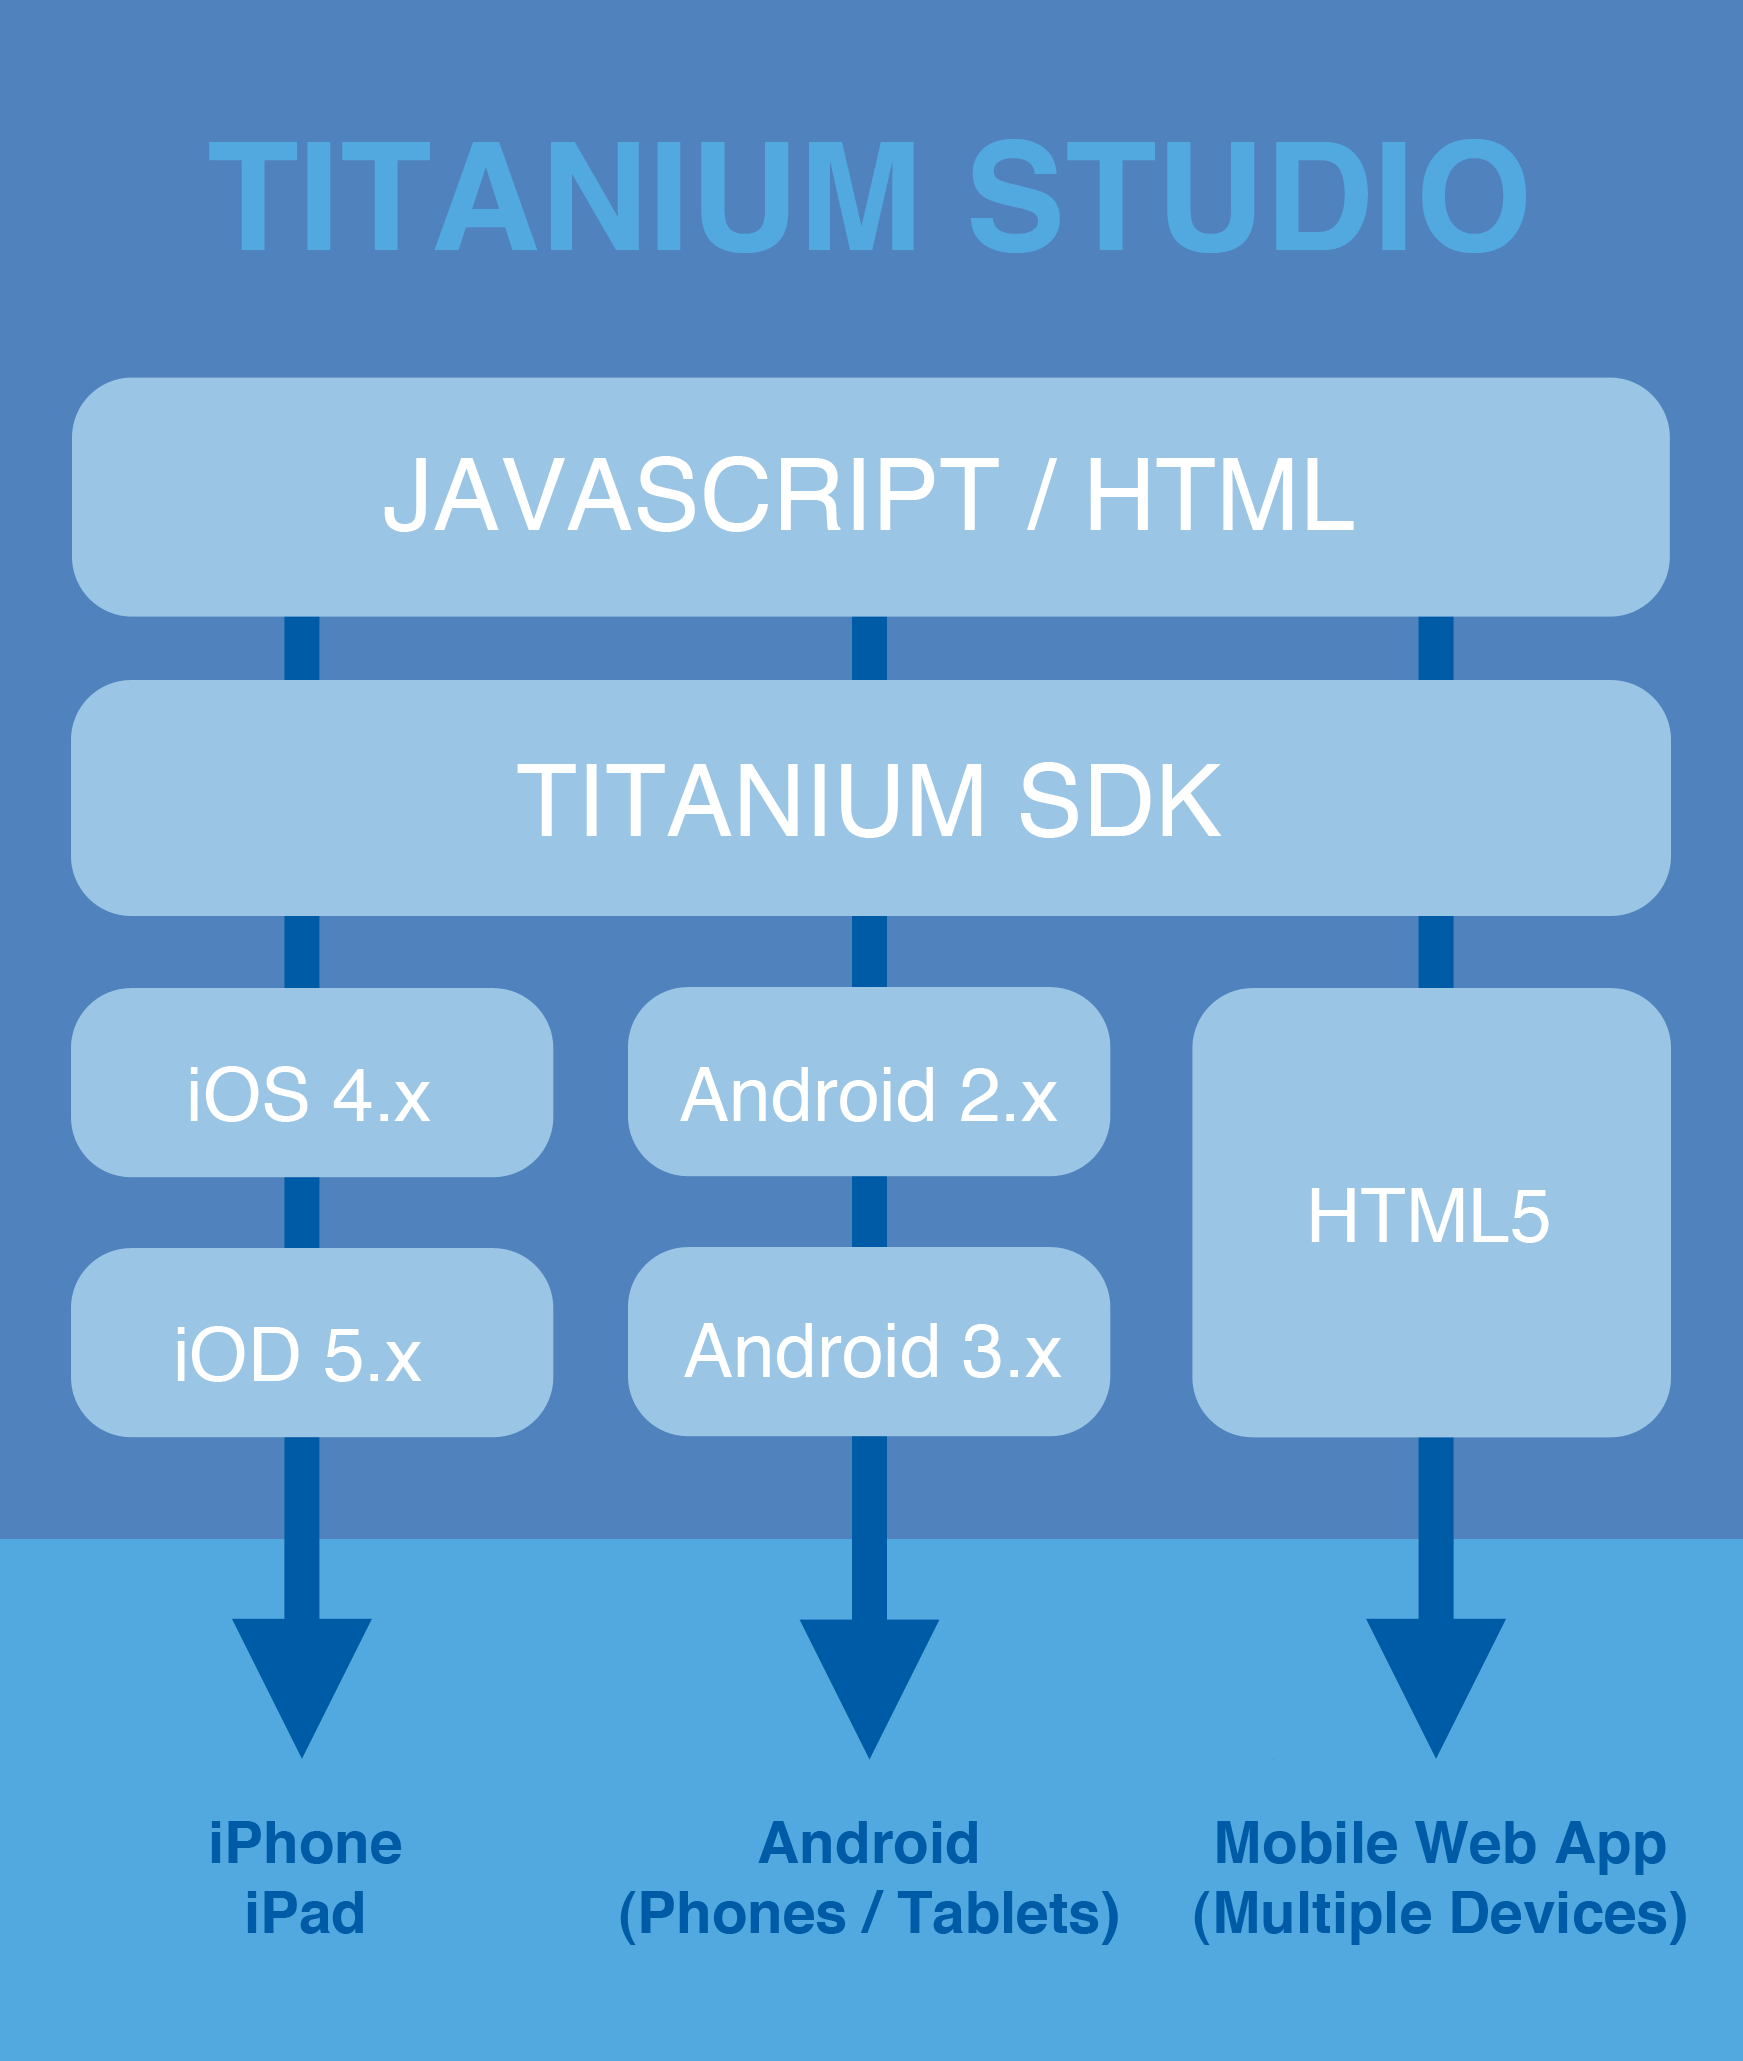
\includegraphics[scale=0.25]{images/titanium_architecture.png}\\{Titaniums bridge architecture\cite{Inc2012a}}\\
\end{centering}

\subparagraaf{Application type}
As mentioned above, Titanium applications are written in JavaScript but can be augmented with HTML \& CSS. The latter is in case a web application is required rather than a native application. This devices applications built with Titanium in two types:
\begin{itemize}
	\item
	Webapplications
	\item
	Native applications
\end{itemize}

\subparagraaf{Philosophy}
The goal of Titanium is to provide a high level, cross-platform JavaScript runtime and API for mobile development.\cite{Whinnery2012} Titanium aims to help developers levarage their JavaScript knowledge to build native mobile apps that run across multiple platforms.




\paragraaf{Rhodes}
Rhodes is an open source Ruby-based framework to build native applications for all major smartphone operating systems (iPhone, Android, RIM, Windows Mobile and Windows Phone 7). These are true native device applications (not mobile web applications) which work with synchronized local data and take advantage of device capabilities such as GPS, PIM contacts and calendar and the camera. %todo: herfomuleren

\subparagraaf{Platform support and native capability}
iOS, Android, BlackBerry, Symbian, Windows Mobile

\subparagraaf{Techniques and tools}
Eclipse based studio, Ruby \& HTML

\subparagraaf{Application type}
Even though Rhodes advertises producing fully native apps\cite{RhoMobile}, they do not. In fact all they do is provide the user with a framework, access to some navigational user interface controls, but the rest is a webview.
\begin{centering}
	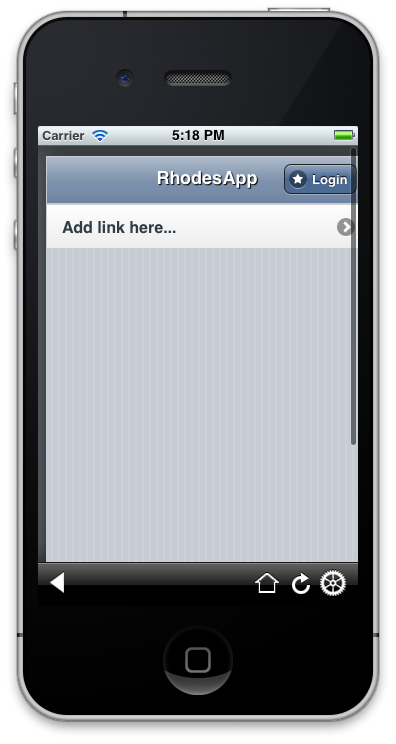
\includegraphics[scale=0.3]{images/rhodes_notsonative.png}\\{Rhodes sample iOS application: not fully native}\\
\end{centering}

\subparagraaf{Philosophy}




\paragraaf{Worklight}
Worklight Studio is an eclipse based IDE for the cross-platform development of mobile applications. Worklight Studio was introduced in 200x by Worklight Inc. In early 2012 Worklight Inc. became an IBM company. Worklight Studio offers mobile development trough the use of webtechnologies such as HTML5, and Javascript.

\subparagraaf{Platform support and native capability}
Worklight supports the following platforms: iOS, Android, BlackBerry and Windows Mobile 7.

\subparagraaf{Techniques and tools}
As mentioned above, Worklight Studio is an eclipse based IDE.
Allows the developer access to device APIs using native code or standard HTML5, CSS3 and JavaScript over a uniform PhoneGap bridge.


\subparagraaf{Application type}
Applications developed with Worklight can be classied as \emph{framework built hybrid applications}. As defined in the previous chapter this means the applications are based fitted inside webview and build on a framework which provides an API to allow the application access to otherwise native API's. The latter is achieved trough Worklights SDK while the former is made possible by an implementation of PhoneGap. \cite{Inc2012}

\begin{centering}
	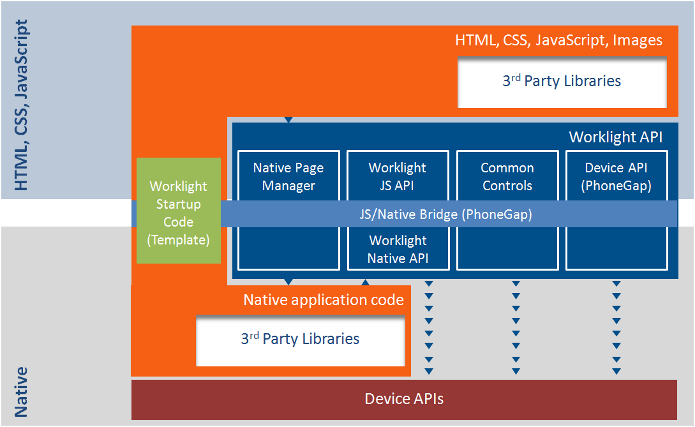
\includegraphics[scale=0.5]{images/Worklight_architecture.png}\\{Worklights bridge architecture\cite{Inc2012a}}\\
\end{centering}

\subparagraaf{Philosophy}
Worklight aims to grant developers access trough HTML5 to the capabilities that mobile devices provide. 


% Modern mobile users want on-the-go access to personalized data and context-driven services delivered at the right time and through the right channel. Augmented reality, Near Field Communication (NFC), push, geo-location, integration with cloud services, and mobile wallets are but a few of the current technologies that enable organizations to streamline operations, reduce costs and increase revenues.

% Worklight was designed from the ground up to address these exact needs. Built around HTML5, Worklight’s open approach does not employ proprietary translators, auto-compilers or esoteric coding languages. Our solution supports multiple development methodologies such as hybrid, web and native, which allow developers to access all of the unique capabilities that modern devices provide.


\paragraaf{MoSync}
The MoSync mobile SDK offers cross-platform development trough the use of webtechnologie or C/C++.

\subparagraaf{Platform support and native capability}

\subparagraaf{Techniques and tools}

\subparagraaf{Application type}

\subparagraaf{Philosophy}


\paragraaf{Comparisson} %todo..

\paragraaf{Conclusion}
%samenvatting geven - misschien hier de overige 3 frameworks al uitsluiten?
